\documentclass[border=10pt]{standalone}

\usepackage{tikz}
\usepackage{tikzsymbols}
\usetikzlibrary{calc,patterns,shapes.geometric}

\def\centerarc[#1](#2)(#3:#4:#5){\draw[#1] ($(#2)+({#5*cos(#3)},{#5*sin(#3)})$) arc (#3:#4:#5);}

\begin{document}
	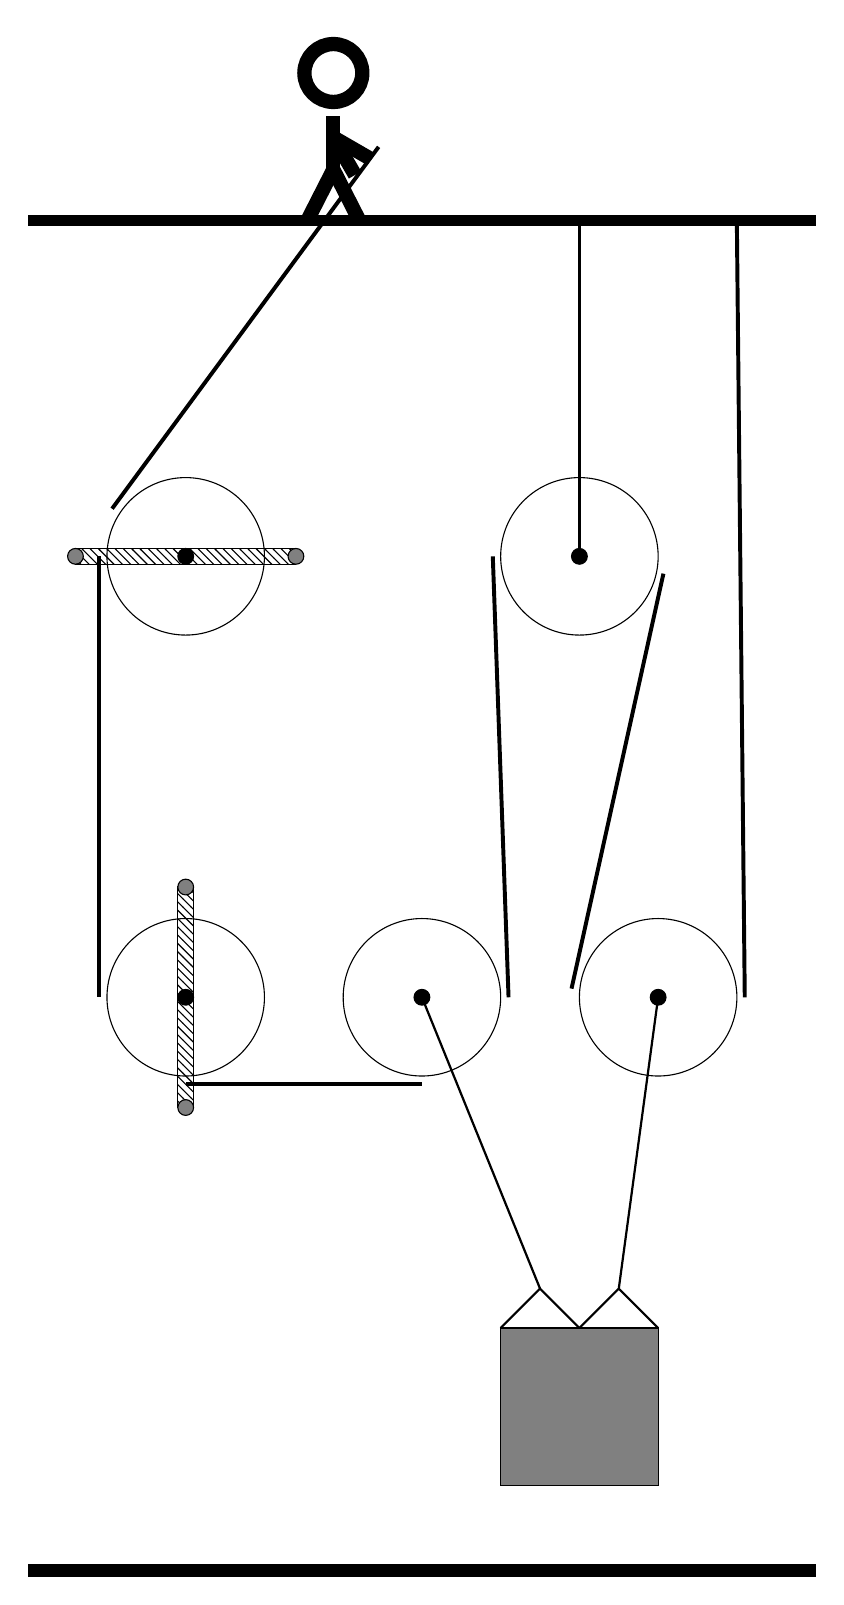
\begin{tikzpicture}
		%%%%% START %%%%%
		\draw[fill=black] (-4, 14) rectangle (6, 14.125);
		
		\draw (1, 4.2) circle (1);
		\draw[fill=black] (1, 4.2) circle (0.1);
		
		\draw (3, 9.8) circle (1);
		\draw[fill=black] (3, 9.8) circle (0.1);
		\draw[thick] (3, 9.8) -- (3, 14);
		
		\draw (4, 4.2) circle (1);
		\draw[fill=black] (4, 4.2) circle (0.1);
		
		\draw[thick] (4, 4.2) -- (3.5, 0.5);
		\draw[thick] (1, 4.2) -- (2.5, 0.5);
		\draw[thick]  (2, 0) -- (2.5, 0.5) -- (3, 0);
		\draw[thick]  (3, 0) -- (3.5, 0.5) -- (4, 0);
		\draw[fill=black!50] (2, 0) rectangle (4, -2);
		
		\draw (-2, 4.2) circle (1);
		\draw[fill=black] (-2, 4.2) circle (0.1);
		\draw[pattern=north west lines, pattern color=black] (-2.1, 5.6) rectangle (-1.9, 2.8);
		\draw[fill=black!50] (-2, 5.6) circle (0.1);
		\draw[fill=black!50] (-2, 2.8) circle (0.1);
		
		\draw (-2, 9.8) circle (1);
		\draw[fill=black] (-2, 9.8) circle (0.1);
		\draw[pattern=north west lines, pattern color=black] (-3.4, 9.9) rectangle (-0.6, 9.7);
		\draw[fill=black!50] (-3.4, 9.8) circle (0.1);
		\draw[fill=black!50] (-0.6, 9.8) circle (0.1);
		
		\draw[line width=0.5mm] (0.45, 15) -- (-2.935, 10.405);
		\centerarc[line width=0.5mm](-2, 9.8)(135:180:1.1);
		\draw[line width=0.5mm] (-3.1, 9.8) -- (-3.1, 4.2);
		\centerarc[line width=0.5mm](-2, 4.2)(180:270:1.1);
		\draw[line width=0.5mm](-2, 3.1) -- (1, 3.1);
		\centerarc[line width=0.5mm](1, 4.2)(270:360:1.1);
		\draw[line width=0.5mm] (2.1, 4.2) -- (1.9, 9.8);
		\centerarc[line width=0.5mm](3, 9.8)(-20:180:1.1);
		\draw[line width=0.5mm](4.067, 9.58) -- (2.9, 4.31);
		\centerarc[line width=0.5mm](4, 4.2)(160:360:1.1);
		\draw[line width=0.5mm](5.1, 4.2) -- (5.0, 14);
		
		\node at (-0.07, 15.2) {\Strichmaxerl[10][120][-30]};
		
		\draw[fill=black] (-4, -3) rectangle (6, -3.15);
		%%%%% END %%%%%
	\end{tikzpicture}
\end{document}